\chapter{Background \& State of the Art} \label{chap:sota}

\section*{}

This chapter has two purposes: describing the foundations on which this work
is built on, namely Machine Learning (ML), Probabilistic Reasoning (PR),
Prograbilistic Programming (PP) and
Visual Programming(VP) while enumerating different tools which are based
on one of these concepts.

\section{Machine learning}

Machine learning (ML) is a field which can be seen as a subfield of artifical
intelligence that incorporates mathematics and statistics and is concerned
with conceiving algorithms that learn autonomously, that is, without human
interventation \cite{mlbrit}\cite{mlnot}.
It has the potential to impact a wide spectrum of
different areas such as biology, medicine, finance, astronomy
\cite{Amatriain:2013:BDU:2541176.2514691}, computer vision, sales forecast,
robotics \cite{intml}, product recommendations, fraud detection or
internet ads bidding \cite{SciPy}.

Learning from data is commercially and scientifically important. ML consists of
methods that automatically extract interesting knowledge in databases of sometimes chaotic and
redundant information. ML is a data-based knowledge-discovering process that
has the potential not only to analyze events in retrospect but also to predict
future events or important alterations \cite{mapt}.

\section{Probabilistic Reasoning}

Probabilistic reasoning (PR) is the formation of probability judgments and of
subjective beliefs about the likelihoods of outcomes and the frequencies of
events \cite{probr}, it is a way to combine our knowledge of a situation
with the laws of probability. There are subjective belifs because, in non-trivial
decision-making there are unobserved factors that are critical to the decision
in conjunction with several sources of uncertainty \cite{reas}, such as:

\begin{itemize}
  \item Uncertain inputs, due to missing or noisy data
  \item Uncertain knowledge, where multiple causes lead to multiple effects,
  or there is an incomplete knowledge of conditions, effects and causality of the
  domain or simply because the effects are inherently stochastic.
\end{itemize}

So, probabilistic reasoning only gives probabilistic results.

It is one way to
overcome cognitive bias and be able to make rational decisions \cite{Sedlmeier2001}.
A trial has been made \cite{christensen1982experience}
where physicians were asked to estimate the probability that a
woman with a positive mammogram actually has breast cancer, given a base rate of
1\% for breast cancer, a hit rate of about 80\%, and a false-alarm rate of about
10\%. It reported that 95 of 100 physicians estimated the probability that she
actually has breast cancer to be between 70\% and 80\%, whereas Bayes's rule
gives a value of about 7.5\%. Such systematic deviations from Bayesian reasoning
have been called "cognitive illusions,". We will describe both Bayes's rules
and Bayesian reasoning in the next section.

\subsection{Bayesian Reasoning}
\label{sec:bayes}

One way to approach PR is by using bayesian reasoning, which is inspired in the
Bayes Theorem (or Rule, or Law). An equivalent formula to the theorem, in its
simplest form (applied to a single event) is:

$$ P(A \mid B) = \frac{P(A \land B)}{P(B)} $$

Where P(A|B) defines the probability of event A given that B occurred.
The theorem defines how hidden causes (A) relate to observed events (B), given
a causality model (P(A, B) or P(B|A)*P(A)) and our knowledge of the probability of the
occurrence of events (P(B)). The inverse is also true, as we will see further
ahead in this section.
As an example, P(penalty | goal) defines the probability that a penalty kick was
scored, knowing that there was a goal.

There are at least two interpretations to the theorem and regarding how one may think
about its results \cite{Fienberg2006}:

\begin{itemize}
  \item Frequentist interpreation: probabilities are defined by the relative
frequency of events, given a natural sampling. Meaning, the probabiltiy of
obtaining 'Heads' when rolling a dice is equal to the number of 'Heads' obtained
after rolling the dice a sufficient number of times relative to the total number
of times the dice has been rolled.
  \item Epistemological interpreation: probabilities represent a measure of
belief. It can either be a result logical combination of probabilities through
the usage of axioms (it's closely related to Aristotlean logic)
or it can also reflect a personal belief (which is called a subjective view).
\end{itemize}

\subsubsection{An example}

One example of the application of this theorem is \cite{reas}: you know your home's alarm
is ringing, but you don't know whether that was caused by a burglar or
something else (maybe a bird triggered it, or there was a malfunction in the
alarm system). How confident are you that you're being robbed? Consider that
the alarm company, based on quality trials, defined in the confusion
matrix for P(alarm, burglary) (Table \ref{tab:bayes}).

\begin{table}[t]
  \centering
  \caption{Alarm system confusion matrix}
\begin{tabular}{| l | l | l |}
	\hline
  & alarm & \neg alarm \\ \hline
 burglary & 0.09 & 0.01 \\ \hline
 \neg burglary & 0.1 & 0.8 \\ \hline
\end{tabular}
  \label{tab:bayes}
\end{table}

You can interpret each table's cell as P(A, B). For instances, the top left
cell is the probability that the alarm rings and there is a burglar, while the
bottom left cell is the probability that the alarm rang but there was no burglar
(a false positive).

If we substitute the values of Bayes' rule described above, we get:

$$ P(burglar \mid alarm) = \frac{P(burglar, alarm)}{P(alarm)} $$

Where results is 0.09 / 0.19 = 0.47. So, even if the alarm is ringing, there is
just a 47\% probability that the house is actually being robbed.

The previous example illustrates the simplest case of applied BR, but it is
also possible to combine several variables.
One way to represent this kind of scenario is by expressing the variables in a directed acyclic
graph, where the relation "Parent" stands for "May cause" and you can specify
the conditional probabilities of a child given a parent's result. This graphical
model is called a Bayesian Network.

\subsubsection{Bayesian Networks}

We can extended our alarm example further, by considering not only a burglar
can trigger the alarm, but an earthquake also can (while there can still be
false positives). Also, consider that we have 2 neighbors (Mary and John) who
may call us whether the alarm is ringing or not. This problem is represented in
figure \ref{beliefnet}.

\begin{figure}[t]
  \begin{center}
    \leavevmode
    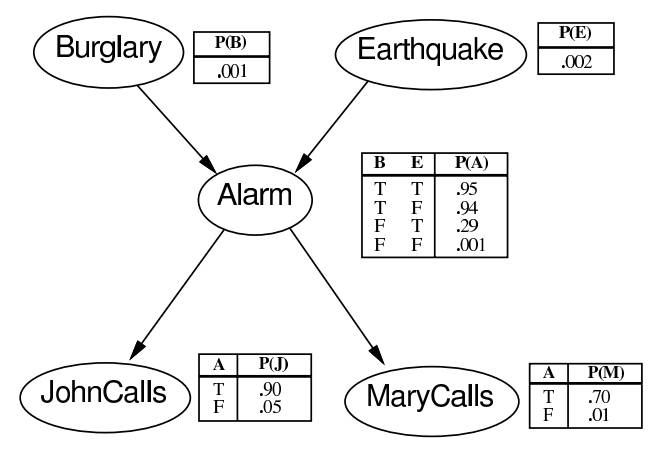
\includegraphics[width=0.86\textwidth]{beliefnet}
    \caption{Belief network for the alarm problem \cite{belfn}}
    \label{fig:beliefnet}
  \end{center}
\end{figure}

Some interesting question we can ask, given this scenario are:

\begin{itemsize}
  \item If John calls saying the alarm is ringing but Mary doesn't, what are the
odds it really is ringing?
  \item If the alarm is ringing, was there an earthquake?
  \item What are the chances that both my neighbors call, the alarm is ringing,
but there is neither a burglary nor an earthquake?
\end{itemize}

This last example, for instances, would be calculated as: P(J, M, A, \neg B, \neg E)
= P(J|A) * P(M|A) * P(A|\neg B, \neg E) * P(\neg B) * P(\neg E) =
0.9 * 0.7 * 0.001 * 0.999 * 0.998 = 0.00062.

Notice how counter-intuitive this
example is: the probability of there being an earthquake is about 32 times larger
then there being an earthquake, the alarm ringing and the neighbors calling us,
even if the conditional probabilities are reasonably high (0.95, 0.9 and 0.7).
This is the result of the calculation of the joint probability being an highly
combinatorial problem, which is yet another argument in favor of using PR
rather than subjective heuristics.

\subsubsection{Bayes' and data streams}

In practical ML applications, it is often the case that there is an
incoming stream of new data, rather than one-time batch calculations.
BR can accomodate this way of thinking, which A. Downey called diachronic
interpretation \cite{thbay}, where diachronic means that something is happening
over time (in this case the probability of the hypotheses, as new data arrives).
In order to make sense of this definition, we may rewrite Bayes' rule as:

$$ P(H \mid D) = \frac{P(D \mid H) \, P(H)}{P(D)} $$

Where:

\begin{itemize}
  \item H: hypothesis
  \item D: data
  \item p(H): probability of the hypothesis before the new data is taken into
account. Also called \textbf{prior}. It can either be calculated using background
information or subjectively defined using domain knowledge. Loses significance
as new data is added, so its choice is not determinant to the model's performance
in the long run.
  \item p(H|D): what we want to calculate, the probability of the hypothesis
after considering the new date. It is called \textbf{posterior}.
  \item p(D|H): probability of the data if the hypothesis was true, called
the \textbf{likelihood}.
  \item p(D): probability of the data under any hypothesis, called the
\textbf{normalizing constant}.
\end{itemize}

Under this interpretation, you may continuously feed data into the model and see
the probabilities getting updated. We will see more practical examples of this
in section \ref{sec:pp}.

\subsubsection{Beyond Bayesian Graphical Model}

At first glance, someone who is learning for the first time about PR applied
to ML, may think that graphical models such as the one presented in Figure
\ref{fig:beliefnet} are the best there can be done in terms of using a graphical
interface for solving this kind of problems and that the only thing is missing
is an automated way to make the calculations.

While it is true we have never refered mentioned techniques or tools that
automatically do inference over a Bayesian Network, there are several tools
with that capability (including an R package \cite{Højsgaard2013} or
standalone tools \cite{msbn}).

However, not all PR can be done via Bayesian Networks and not all graphical models
are enough for complete PR \cite{intpp}. PP are the largest class of models available, and there are
also more algorithms for inference than just the calculation of joint
probabilities (like we did in the alarm example), as we will discuss in Section
\ref{sec:pp}.

Bayesian Networks are not the only kind of graphical model. Another one would be
Markov Chains, which is yet another example of a model which is not able to
represent all PR problems. This is clear when we realize that, while PPLs
support a large number of different distributions (such as Normal, Laplace,
Gamma, Half-Cauchy or \textit{t}), all Bayesian Networks and Markov Chain
can be represented in a PPL by just using Bernoulli distributions \cite{PPm}.
We can see an example of such a translation in Figure \ref{fig:mppl}.

\begin{figure}[t]
  \begin{center}
    \leavevmode
    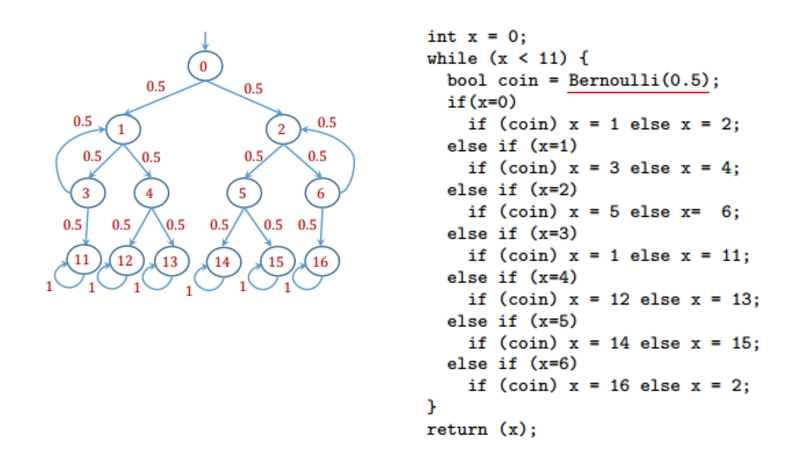
\includegraphics[width=0.86\textwidth]{markppl}
    \caption{Translation of Discrete Time Markov Chain to a PPL \cite{PPm}}
    \label{fig:mppl}
  \end{center}
\end{figure}

<---- rever com base em prob inference for graphical models

\subsection{Probabilistic Programming Languages}
\label{sec:pp}

\subsubsection{The Probabilistic Program-Model duality}

A probabilistic program (PP) is an ordinary program (that can be written in
mainstream languages such as C, Java or Haskell) whose purpose is to specify
a probability distribution of its variables. This is done by sampling over
several executions of the program. The only needed construct the language
has to support, in order to be able to write a PP, is having a random number
generator \cite{Duvenaud}. This whole concept couldn't be better explained than in this text by Freer and
Roy, regarding Church (a PPL, which we describe in Section \ref{sec:church})
but common to any PP:

\begin{quote}
  ``If we view the semantics of the underlying deterministic language as a map
  from programs to executions of the program, the semantics of a PPL built on it
   will be a map from programs to distributions over executions. When the
   program halts with probability one, this induces a proper distribution over
   return values. Indeed, any computable distribution can be represented as the
   distribution induced by a Church program in this way''~\cite{Freer2012}
\end{quote}

One way to think about this notion is by considering that the program itself
is the model. An example of the relation between a model (expressed in a PPL)
and the implied distribution over its variables (obtained using an inference
method) can be seen in Figure \ref{distribution}, where a variable \textit{flip}
is set to be a Bernoulli distribution and \textit{x} is defined in terms of
\textit{flip}. We can then see how the graphic of the inferred distributions
of \textit{flip's} and \textit{x's} values looks like and confirm what was to
be expected: for \textit{flip's} values lower than 0.5 we see \textit{x} follows
a normal distributon, whereas for values greater than 0.5 it follows a gamma
distribution instead.
 The goal of PP is to enable PR and ML to be accessible to
most programmers and data scientists who have enough domain and programming
knowledge but not enough expertise in probability theory or machine learning.

\begin{figure}[t]
  \begin{center}
    \leavevmode
    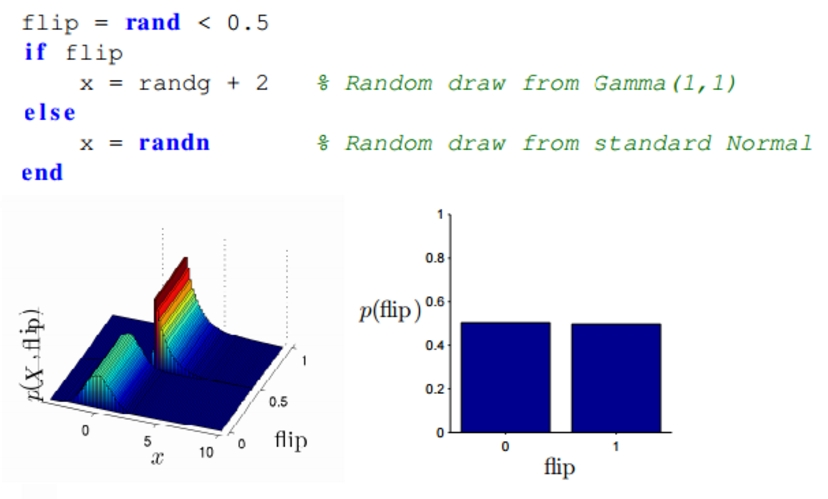
\includegraphics[width=0.86\textwidth]{distribution}
    \caption{Implied distributions over variables \cite{Duvenaud}}
    \label{fig:distribution}
  \end{center}
\end{figure}

\subsubsection{PPLs vs regular PLs}

What is then, a Probabilistic Programming Language (PPL)? First of all, it can
be a standalone language or an extension to a general purpose programming languag.
We'll be analyzing examples of languages from either these categories in Section
\ref{sec:art}, but many more exist, such as as Figaro \cite{figaro} (hosted in Scala),
webppl \cite{dippl} (embedded in Javascript) or Dimple
\cite{DBLP:journals/corr/abs-1212-2991} (has both a Java and a MATLAB API).
The key difference between these languages and a PPL is the latter has
the added capability of performing conditioning and inference \cite{Andrieu2003}.

Conditioning is the ability to introduce observations about the real world in
the program. That way, you update the prior probability based
on those observations. Consider the example in Figure \ref{fig:truskill} (which
is a simplified version of how Microsoft applies PP in its Xbox matchmaking
algorithm \cite{minka2012infer}) where the prior is a normal distribution with
equal parameters for all players (shown by the graphic in the top). Then, it
defines how the performance of the player is based on his skill (which at the initial
point in time, is equal to every one of them) and proceeds to make several
observations regarding games between them. Finally, it shows the inferred
probability distribution of the posterior on the bottom graphic.

\begin{figure}[t]
  \begin{center}
    \leavevmode
    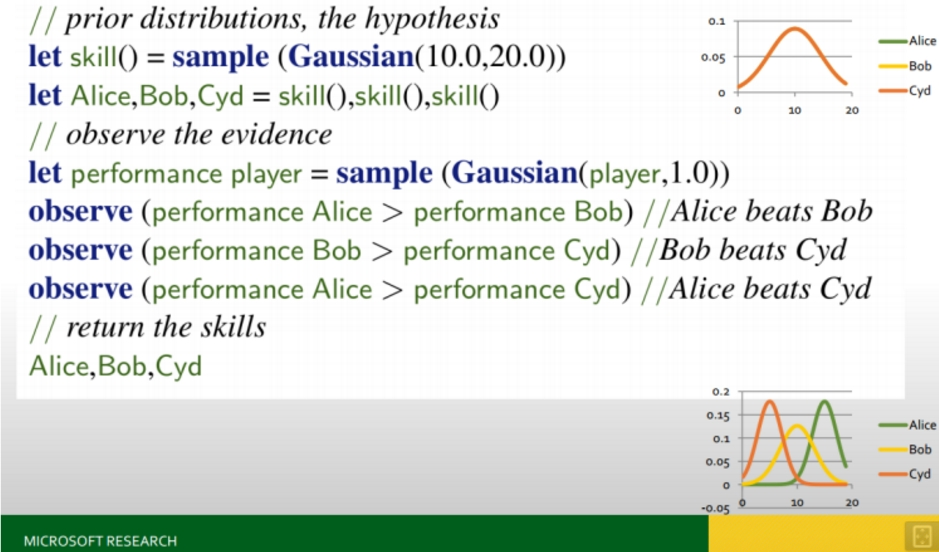
\includegraphics[width=0.86\textwidth]{trueskill}
    \caption{Microsoft Xbox Live True Skill \cite{minka2012infer}}
    \label{fig:truskill}
  \end{center}
\end{figure}

\subsubsection{Inference}

We said that a PPL empowers the user to formalize a model and then query for the
probability distribution of its variables, which is automatically done via
inference. While general-purpose language require you to write one-time
inference methods that tightly coupled to the PP you are inferring on, PPLs
ship with an inference engine suited to most PP programs you can write
\cite{Freer2010}.

An inference engine of a PPL acts similarly to a compiler in a traditional
language: rather than requiring each user to engineer its own, which requires
significant expertise and is a non-trivial and error-prone endeavour, every PPL
has one incorporated. Olivier Grisel called this separation of concerns
between the language and its inference engine "openbox models, blackbox
inference engine" \cite{SciPy}.

Having the engine work as a separate model opens up a myriad of new
possibilities, mainly in the form of knowledge and tool sharing, as we have
seen in the past in the compiler space. Examples of this would be new compiler
compiler and interpreter techniques (such as working towards scalability or
parallelization), optimizers, profilers or debuggers.

Another great advantage of having a modular inference engine is that we can
try different inference algorithms and pick the one that best fits the problem
at hand. When analyzing if algorithm suits a certain use case, there are certain
characteristics worth noting \cite{Minka1999}:

\begin{itemize}
  \item Determinism - in equal initial conditions, an algorithm always yields
the same result.
  \item Exact result or approximation
  \item Guaranteed convergence - an algorithm may or not be guaranteed to reach
a result at some point in time. If not, it's possible that it will run forever.
  \item Efficiency - related to how fast can it reach a result.
\end{itemize}

Microsoft's Infer.NET provides three inference algorithms \cite{msalg}:

\begin{itemize}
  \item Expectation Propagation - deterministic, provides exact solutions only
in some cases, is not guaranteed to converge and is labelled as "reasonably
efficient".
  \item Variational Message Passing - also deterministic, but always gives
approximates results and is guaranteed to converge. It's considered to be the
most efficient of the three for most cases.
  \item Gibbs sampling - non-determinisc, may be able to reach exact result
if given enough time to run, has guaranteed convergence and is regarded as
not-so-efficient as the other two.
\end{itemize}

We can divide the three algorithms into two categories: variational bayesian
methods \cite{Winn2005}\cite{Minka1999} and sampling methods (in the case of Gibbs
sampling, it's based on Markov chain Monte Carlo) \cite{Andrieu2003}. The main
difference, as far as the end-user is concerned, is that variational methods
provide faster results but are subject to bias, whereas sampling methods have
the potential to produce more accurate results (the downside being it's slower
and its convergence is hard to diagnose) \cite{Shen2010}.

Please notice than none of these algorithms provides the same kind of exact
solution as the calculation of the joint probabilities we did in Section
\ref{sec:bayes}. The reason for that is that calculating an exact solution
takes time exponential in the number of variables to run, even if we have smarter
algorithms than the naive calculations we did \cite{Zhang1994}.

\subsubsection{Openbox models}

When compared to traditional machine learning methods (such as random forests, neural
networks or linear regression), which take homogeneous data as input (requiring
the user to separate their domain into different models), probabilistic
programming is used to leverage the data’s original structure. This is done by
empowering the user to write his own models while taking advantage of a re-usable
inference engine. Olivier Grisel called this combination "Openbox models,
blackbox inference engine"\cite{SciPy}.

Rather than using most of his
time performing feature engineering (that is, trying to fit the problem and the
data into an existing model), the user will have the tool necessary to design
the model that best fits the domain he is working on.
Plus, it provides full probability distributions over both the predictions and parameters of the
model, whereas ML methods can mostly only give the user a certain degree of confidence
on the predictions.

\subsection{Conclusion}

Summarizing, PPLs are a step forward in using PR to solve ML problems since
it helps overcome the difficulties in using PR in real world problems. This is
done by adding automated general inference on top of a precise specification
(the program), where in the past models were communicated
using a mix of natural language, pseudo code, and mathematical formulae and solved
using special purpose, one-off inference methods.

This encourages exploration, since
different models require less time to setup and evaluate, and enables sharing
knowledge in the form of best practices and design and development patterns.

However, using a full fleged programming language might still be an entry
barrier. We want to help statisticians and data scientists alike to learn
faster and be more productive using a PPL in a way similar to the tools they
are accostumed to. In order to do so, we'll be combining a PPL with Visual
Programming (Section \ref{sec:vp}).

\section{Visual Programming}
\label{sec:vp}

Visual Programming (VP) can be defined as "any system that allows users to
represent "any system that allows the user to specify a program in a
two-(or more)-dimensional fashion." \cite{Myers1986}.
In a textual programming language, even though there are two dimensions (one
being the text itself, and the other the optional line-breaking characters),
only one of them has semantics, as the compiler processes text as a
one-dimensional stream.

Examples of systems with aditional dimentions are ones that allow the use of
multidimensional objects, the use of spatial relationships, or the use of the
time dimension to specify “before-after” semantic relationships \cite{Burnett1999}.

Research has identified several advantages in the use of VP, such as natural
expressibility, easy readability and interaction, language independence (though
this is not applicable to the work of this thesis, as detailed in \ref{sec:vpe}),
programming at higher levels of abstraction or rapid prototyping \cite{JamalRahmanandWenzel2014},
which is achieved by providing immediate visual feedback \cite{Shu1988}.

The advantages of programming at highers levels of abstraction are known, and
one of them is it exposes users who are not used completely fluent in programming
to a reduced number of concepts \cite{Shu1988}, while decreasing the verbosity of
programs, which can even be useful for seasoned programmers \cite{Myers1990}.
It also reduces the importance of being familiar with syntax, a common cause
of difficulty of adaptation among less experienced programmers when learning
a new language \cite{cunniff1986does}\cite{Carlisle2005}. This difficulty of translating ideas
into syntactictically correct statements can also be solved by finding alternative
ways to communicate instructions to the computer \cite{Kelleher2005}.

So, the point of using a VP tool to aid in programming is to overcome the
difficulties that many people have when learning a conventional language
\cite{Lewis1987}. It has been shown this approach can help users without prior, or little,
programming experience to create fairly complex programs \cite{Halbert1984}.
This is specially true within certain small domains, where the language can be
tailored for a subset of tasks rather than trying to be suitable for all kinds
of applications \cite{Kelleher2005}. An example of such domain would be
developing ML applications resorting to probabilistic programming.
Excel-like (spreadsheet) tools are a prime example of this, where the following
benefits were identified \cite{ambler1987forms}\cite{empstud}:

\begin{itemize}
  \item The graphics on the screen use a familiar, concrete, and visible representation which
directly maps to the user’s natural model of the data
  \item They are non-modal and interpretive and therefore provide immediate feedback
  \item They supply aggregate and high-level operations
  \item They avoid the notion of variables (all data is visible)
  \item The inner world of computation is suppressed
  \item Each cell typically has a single value throughout the computation
  \item They are non-declarative and typeless
  \item Consistency is automatically maintained
  \item The order of evaluation (flow of control) is entirely derived from the declared cell dependencies
\end{itemize}

Smith and other authors claim that the human thought process is clearly optimzed
for multi-dimensional data \cite{smith1977pygmalion}\cite{Clarisse1986},
so all the aforementioned advantages can be explained by how graphical programming is closer
to our mental representation of problems when compared to a textual interface
\cite{Cardellini2002}. As said by Fischer, Giaccardi, Sutcliffe and Mehandjiev:

\begin{quote}
  ``Text-based languages tend to be more complex because the syntax and lexicon
  (terminology) must be learned from scratch, as with any human language.
  Consequently, languages designed specifically for end users represent the
  programmable world as graphical metaphors ... (\textit{aim to}) reduce the cognitive
  burden of learning by shrinking the conceptual distance between actions in
  the real world and programming.'' \cite{G2004}
\end{quote}

This idea as been tested in an empirical study:
in a algorithms course of the United States Air Force academy,
students consistently show a preference for solving problems visually,
while it also seems that doing so helped them achieving better
scores in problem-solving exercises and overperform their colleagues who used
a regular programming language \cite{Cardellini2002}. However, shortcomes of
using VP were also identified, as we will discuss in \ref{sec:crit}.

\subsection{Visual Programming Environment}
\label{sec:vpe}

Boshernitsan proposed a classification scheme for VPLs \cite{Boshernitsan2004}
that divided VPLs in purely visual languages (PVLs), hybrid text and visual systems,
programming-by-example systems, constraint-oriented systems and form-based systems.

In the context of this dissertation, as we want to leverage the advantages of
both a VPL and a PPL while avoiding implementing a PPL, there is no other choice
than using an hybrid text and visual system. We will be calling this system a
visual programming environment (VPE). The difference between a VPE and a purely visual language (PVL)
is that, while a PVL is a language \textit{per se} (meaning that it there
is a direct mapping between graphics and execution), VPEs offer a middle ground
between regular textual languages and PVLs: they provide a graphical interface
that can be used to generate code for a target language \cite{Burnett1999}.
An example of a PVL would be MIT's Scratch \cite{resnick2009scratch} and one for
a VPE is the Eclipse IDE plug-in WindowBuilder \cite{winbuild}.

If applied
correctly, VPEs can help addressing some of the issues raised by critics of VP (detailed in section \ref{sec:crit}),
such as VP's inhability to solve real-world, large-scale problems. This is done
by applying VP to only a subset of the program, making it possible to combine
a general-purpose programming language with the advantages of VP \cite{Burnett1999},
since the code generated by a VPE can be seseamlessly integrated in any project
built with its target language.

Concretely, VPEs are able to overcome the tradeoff of control for simplicity
commonly made by VPLs: even if a certain idiom cannot be represented by its
graphical form, the user can later edit the generated code to include it. This
makes it possible to design scalable programs, both in terms of performance
(since the user can still access all the target language's features) and development
(because all the advantages of programming visually are still present).

\subsection{Assessing the impact}

Na teoria \cite{Burnett1999}
Na pratica \cite{Whitley1997}

Visual Programming:
The Outlook from Academia and Industry K.

A estudar impl ler "controlled dataflow vpl"

\subsection{Challenges}

Scaling up

\subsection{Criticism}
\label{sec:crit}

programming languages is the lack of visual abstraction mechanisms that are as = effective as those offered by text?based languages
Thus, it is generally considered that traditional programming languages are better suited for developing large applications

an integrated graphical user interface promote the iterative design and interactive prototyping,
often including simulation in early stages of development.
This melding of development and execution can be considered as one of the major
benefits of a graphical programming environment,
where the edit/compile/link/run sequence of traditional programming languages is replaced by the draw/run cycle.
In addition, it has been shown that the richness of the visual paradigm
introduces new ways of approaching programming problems, particularly for
those not trained in traditional software development methods

(resposta: An early effort that was not based on flowcharts was the AMBIT/G [25] and AMBIT/L [26] graphical languages. They supported symbolic manipulation programming using pictures.
Both the programs and data were represented diagrammatically as directed graphs, and the programming operated by pattern matching. Fairly complicated algorithms, such as garbage col- lection, could be described graphically as local transformations on graphs.
\cite{Myers1990})
\cite{JamalRahmanandWenzel2014}

(i) Is VP any good? Although lab studies have not produced much evidence in its favour, some people like and use VPLs. Visual tracers likewise. So the lab studies have missed something. What? (Maybe it’s fun, like a video game.)
(ii) Does the visual component really contribute anything extra? Sometimes ‘visual’ systems do nothing that can’t be done as well or better with straight text; perhaps the real issues are how layout and locality can be used to convey meaning [
\cite{Shu1988}

A favorite subject for PhD dissertations in software engineering is graphical, or visual,
programming—the application of computer graphics to software design....
Nothing even convincing, much less exciting, has yet emerged from such efforts. I am persuaded that nothing will. In
the first place, ... the flowchart is a very poor abstraction of software structure....
It has proved to be useless as a design tool.... Second, the screens of today are too small, in pixels, to show both
the scope and the resolution of any seriously detailed software diagram.... More fundamentally, ...
software is very difficult to visualize. Whether one diagrams control flow, variable-scope nesting,
variable cross-references, dataflow, hierarchical data structures, or whatever, one feels only one
dimension of the intricately interlocked software elephant.
\cite{Brooks1986}

I was recently exposed to ... what ... pretended to be educational software for an introductory programming course.
With its ‘‘visualizations’’ on the screen, it was ... an obvious case of curriculum
infantilization.... We must expect from that system permanent mental damage for most students
exposed to it.
\cite{dijkstra1989cruelty}

Visual Languages are new paradigms for programming, and clearly the existing systems have
not been completely convincing. The challenge clearly is to demonstrate that Visual Programing
and Program Visualization can help with real-world problems. The key to this, in my
opinion, is to find appropriate domains and new domains to apply these technologies to.

successful so far: allowing non-programmers to enter information in limited domains

problems:
\begin{itemize}
  \item Difficulty with large programs or large data. Almost all visual representations are physi-
cally larger than the text they replace, so there is often a problem that too little will fit on
the screen. This problem is alleviated to some extent by scrolling and various abstraction mechanisms.
  \item Need for automatic layout. When the program or data gets to be large, it can be very tedi-
ous for the user to have to place each component, so the system should lay out the
picture automatically. Unfortunately, for many graphical representations, generating an
attractive layout can be difficult, and generating a perfect layout may be intractable. For
example, generating an optimal layout of graphs and trees is NP-Complete [95]. More
research is needed, therefore, on fast layout algorithms for graphs that have good user
interface characteristics, such as avoiding large scale changes to the display after a small
edit.
  \item Lack of formal specification. Currently, there is no formal way to describe a Visual
Language. Something equivalent to the BNFs used for textual languages is needed. This
would provide the field with a ‘‘hard science’’ foundation, and may allow tools to be
created that will make the construction of editors and compilers for Visual Languages
easier. Chang [49] [96], Glinert [97] and Selker [98] have made attempts in this
direction, but much more work is needed.
  \item Tremendous difficulty in building editors and environments. Most Visual Languages
require a specialized editor, compiler, and debugger to be created to allow the user to use
the language. With textual languages, conventional, existing text editors can be used and
only a compiler and possibly a debugger needs to be written. Currently, each graphical
language requires its own editor and environment, since there are no general purpose
Visual Language editors. These editors are hard to create because there are no ‘‘editor-
compilers’’ or other similar tools to help. The ‘‘compiler-compiler’’ tools used to build
compilers for textual languages are also rarely useful for building compilers and
interpreters for Visual Languages. In addition, the language designer must create a system to
display the pictures from the language, which usually requires low-level graphics
programming. Other tools that traditionally exist for textual languages must also be created,
including pretty-printers, hard-copy facilities, program checkers, indexers,
cross-referencers, pattern matching and searching (e.g., ‘‘grep’’ in Unix), etc.
These problems are made worse by the historical lack of portability of most graphics programs.

  \item Lack of evidence of their worth. There are not many Visual Languages that would be
  generally agreed are ‘‘successful,’’ and there is little in the way of formal experiments or
informal experience that shows that Visual Languages are good. It would be interesting
to see experimental results that demonstrated that visual programming techniques or
iconic languages were better than good textual methods for performing the same tasks.
Metrics might include learning time, execution speed, retention, etc. Fortunately, prelim-
inary results are appearing for the advantages of using graphics for teaching students how
to program [36].
  \item Poor representations. Many visual representations are simply not very good. Programs are
hard to understand once created and difficult to debug and edit. This is especially true
once the programs get to be a non-trivial size.
  \item Lack of Portability of Programs. A program written in a textual language can be sent
through electronic mail, and used, read and edited by anybody. Graphical languages
require special software to view and edit; otherwise they can only be viewed on hard-copy
\end{itemize}
\cite{Myers1990}

Of note here is the observation that this conclusion did not extend to the use of arrays in problem solving.
In fact, the first semester with RAPTOR students performed statistically significantly worse on the array question.
This would suggest that array handling in RAPTOR might be an area for future improvements.
\cite{Cardellini2002}

solução: para ultrapassar problemas comuns de VP em sistemas reais, larga-escala,
usar apenas VP em partes especificas do projeto onde VP possa ser utilizado com
sucesso. usar para desenhar GUIs foi um sucesso (android, windowbuilder)

fazer programar mais facil para audiencia especifica
\cite{Burnett1999}

\section{State of the Art}
\label{sec:art}

\subsection{Stan}

\subsection{WinBUGS}
\label{sec:wbugs}

\subsection{Church}
\label{sec:church}

\subsection{Infer.NET}

\subsection{PyMC}

\subsection{VIBES}

\subsection{NoFlo}

\subsection{RapidMiner}

\subsection{Weka Knowledge FLow}

\subsection{GoJS}

\subsection{Blockly}

\section{Conclusions}
